\section{Applying the platform to the OLAF problem}

The problem of creating an address file for the UK was described in chapter \ref{subs:the-problem-of-creating-an-olaf}. This section describes a possible workflow that can be implemented on the platform and how some of its parts were implemented for evaluation.

\subsection{How primary open data sources shape the problem}

The availability of reliable relevant open data is central to the definition of the workflow, as it is the main assumption of the work that the best possible use of computation and crowdsourcing is to complement published data rather than creating it from scratch [I THOUGHT I HAD WRITTEN THIS IN THE DOCUMENT BEFORE, WHERE IS IT?]. 

An assessment of what open data sources were available, made at the time this work was performed, made it possible to consider solving the OLAF problem equivalent to solving three sub-problems {\it p1}, {\it p2} and {\it p3} as shown in figure \ref{fig:problem_decomposition_1}, focused on enhancing the same open dataset: Ordnance Survey's "Open Names"\footnote{Ordnance Survey is the national mapping agency for Great Britain. See \url{https://www.ordnancesurvey.co.uk/business-and-government/products/os-open-names.html}.}, (referred to as "OSON" in the following).

\begin{figure}
	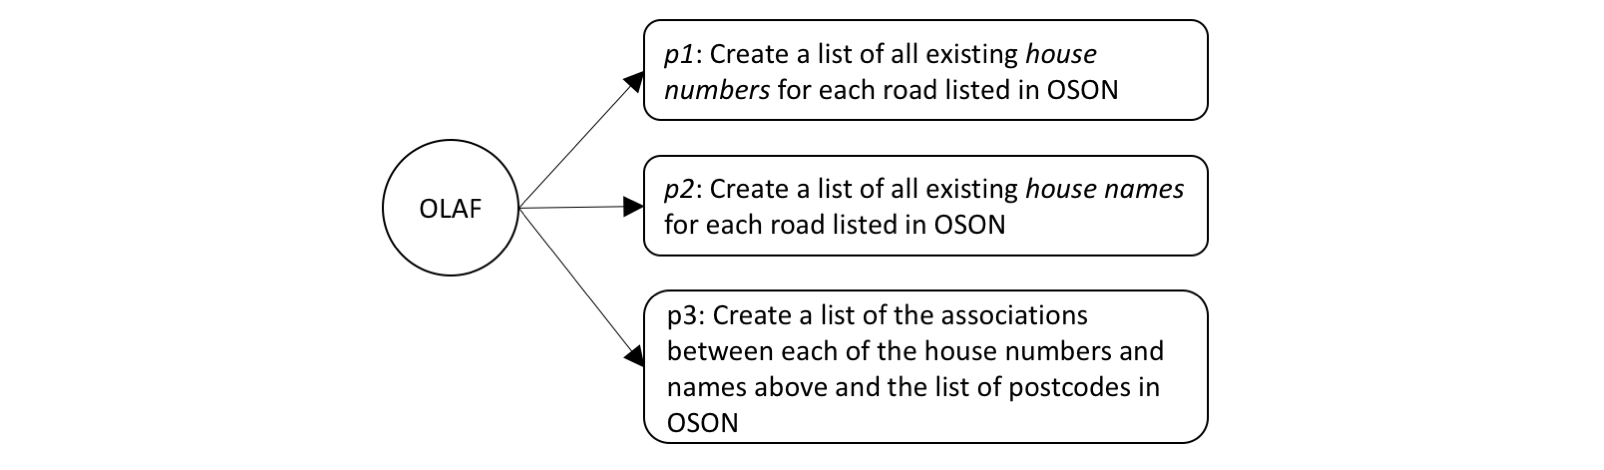
\includegraphics[width=1.0\textwidth]{problem-decomposition-1.png}
	\caption{A possible decomposition of the OLAF problem - First level}
	\label{fig:problem_decomposition_1}
\end{figure}

OSON "lists definitive place names, roads numbers and postcodes in Great Britain" and is instrumental to the work as it is the open dataset that is closer to the target, contentwise. In other words, OLAF can be seen as an augmentation of OSON, obtained by adding just one dimension to what can be already found in it, that is the list of house names and numbers associated to each of its roads and postcodes. 
    
Problems {\it p2}\footnote{Note that 98\% of UK addresses are characterised by a house number rather than a house name, so solving {\it p1} is substantially more relevant to achieve completeness in OLAF than {\it p2}.} and {\it p3} are not discussed further in this document. 

Problem {\it p1} can be further decomposed in four sub-problems as shown in figure \ref{fig:problem_decomposition_2}, thanks to the availability of additional open data sources and Land Registry's "Price Paid Data"\footnote{Land Registry is a non-ministerial UK Government department with the responsibility to register the ownership of land and property in England and Wales. See \url{https://www.gov.uk/government/collections/price-paid-data}.} ("LRPP" in the following) in particular.
    
\begin{figure}
	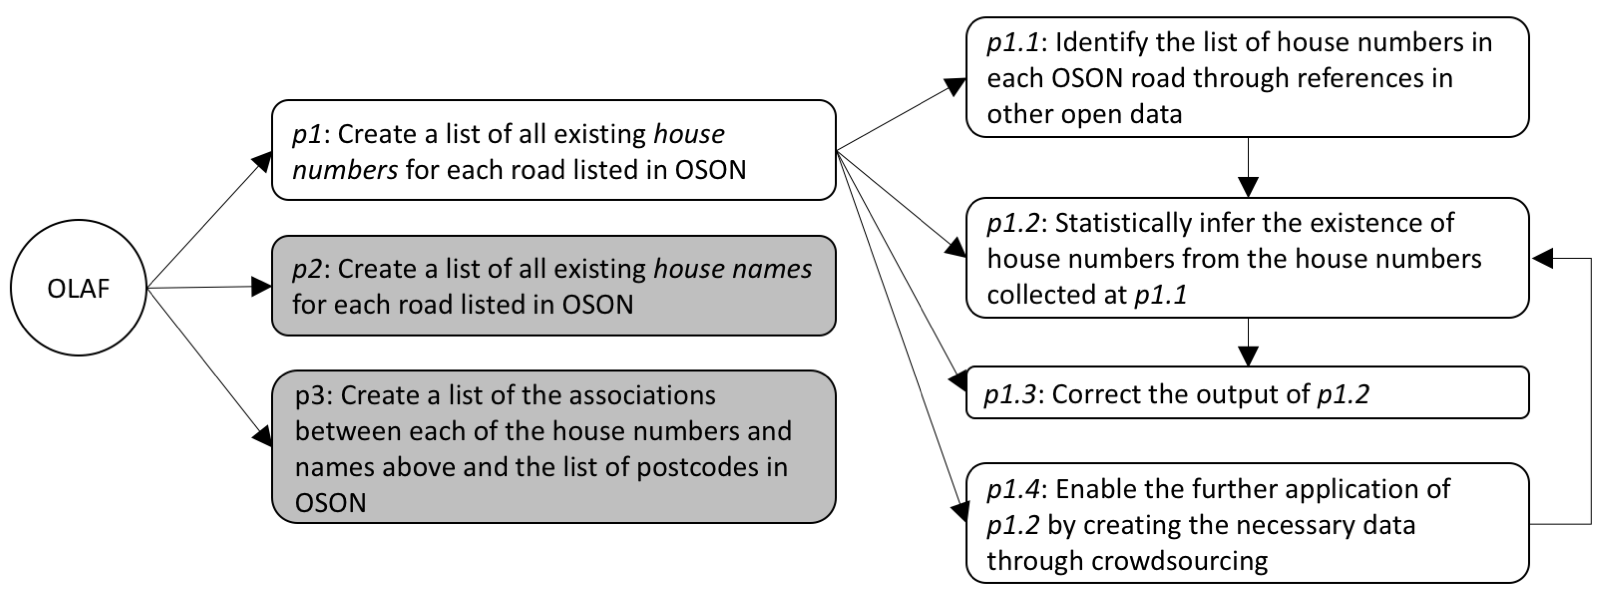
\includegraphics[width=1.0\textwidth]{problem-decomposition-2.png}
	\caption{A possible decomposition of the OLAF problem - First and second level}
	\label{fig:problem_decomposition_2}
\end{figure}

Problem {\it p1.3} is not discussed in this paper\footnote{Error in inferred house numbers is caused by three situations: (i) inferred house numbers for buildings that use house names instead (ii) inferred house numbers that in reality exist only in suffixed form (e.g. 7A instead of 7), and (iii) addresses that are simply missing, e.g. because a building was demolished. The volume of errors is considered not sufficient to compromise the use of inference. E.g. it can be calculated for (i) that the frequency of addresses identified by house names instead than house numbers is only 2\% of the total for the sampled geographic area. For (ii), the probability that a house number is used only in suffixed format is estimated to be 2.6\%, and that it is used {\it also} in suffixed format an additional 4.1\%. This is like saying that, out of 50 inferred house numbers, (i) 1 is in reality a house name, (ii) 2 are correct but are missing the suffixed variations and 1 is does not exist and should be replaced by its suffixed variations. Moreover, this is a worst case scenario, as the sample we used for the estimates is heavily urbanised.}.

\subsection{Creating a list of all existing house numbers for each road listed in OSON} 

LRPP records every property ownership transfer in England and Wales since 1995, including their full addresses. It is just one of the several open data publications in the UK that include addresses, and the largest in size, hence particularly suitable to be used in the experiments.

Although the streets referenced in LRPP may not necessarily exactly match the ones in OSON (e.g. because of slightly different spelling) it is possible to identify most of them without manual intervention and with a good degree of confidence to collect the house numbers as needed.

\subsection{Inferring the existence of house numbers} 

\textbf{Numbering convention} Inferring house numbers is strictly dependent on the numbering convention for the assignment of house number and names to building. Each culture developed its own over time. In the UK, buildings are typically numbered sequentially starting from 1, corresponding to the extremity of the road that is closest to the centre of the town the street belongs to. Odd numbers are on the left-hand side as seen from the centre, even number on the right-hand side. Intermediate properties usually have a number suffixed by one or more letters, this is typical of larger buildings that at some point in time got divided into more smaller dwellings. 
        
\textbf{Inference algorithms} Algorithms \ref{algo:inference-numbers} and \ref{algo:inference-numbers-suffix} below apply this understanding of the numbering system and have a very high probability to infer correctly the existence of house numbers from other known house numbers\footnote{It should be remembered, though, that centuries of house development and using the described numbering system loosely of course created many exceptions: e.g. there are buildings in the UK whose house number is zero, places where numbers were assigned consecutively on the same side of the street, and house numbers that are simply missing etc. Other available open data sources enable more complex algorithms, e.g. Ordnance Survey's "Open Maps - Local" includes summary shapes for the buildings in each street, hence enabling the detection of how many buildings are present and hint at which house numbers may be missing.}. Although a few house numbers will be inferred in error, .

\vspace{5mm}

\begin{algorithm}[H]
    \KwData{The list of known house numbers in a road}
    \KwResult{The list of inferred house numbers in the same road}
    \eIf{the list includes at least one even and one odd number}{
        infer all numbers between the lowest and the highest known numbers\;
    }{
        \If{the list includes at least two even or two odd numbers}{
            infer all even/odd numbers between the lowest and the highest numbers\;
        }
    }
    \caption{Inference of house numbers}
    \label{algo:inference-numbers}
\end{algorithm}

\vspace{5mm}

\begin{algorithm}[H]
    \KwData{The list of known house numbers with suffixes in a road}
    \KwResult{The list of inferred house numbers with suffixes in the same road}
    \For{each house number appearing in the list with at least two suffixes}{
        infer all suffixes between the lowest and the highest known suffix, in alphabetical order\;    
    }
    \caption{Inference of house number with suffixes}
    \label{algo:inference-numbers-suffix}
\end{algorithm}

\subsection{Enabling the further application of the inference algorithms} 

It is evident from the specification of the algorithms that the inference of house numbers is enabled one of these two conditions: (a) the knowledge of two or more different house numbers in the same street and (b) the knowledge of two or more suffixes for the same number.

\textbf{Potential of inference} 82\% of the streets in scope are referenced in LRPP. Executing the inference algorithms on the house numbers sourced from {\it p1.1} creates opportunities for inference for the 74\% of roads and ~113k house numbers. If more house numbers were known, inference could be applied to both (i) further populate streets where inference was already applied and (ii) apply inference for the very first time to streets we know nothing about.

\begin{figure}[!ht]
    \begin{floatrow}
        \ffigbox{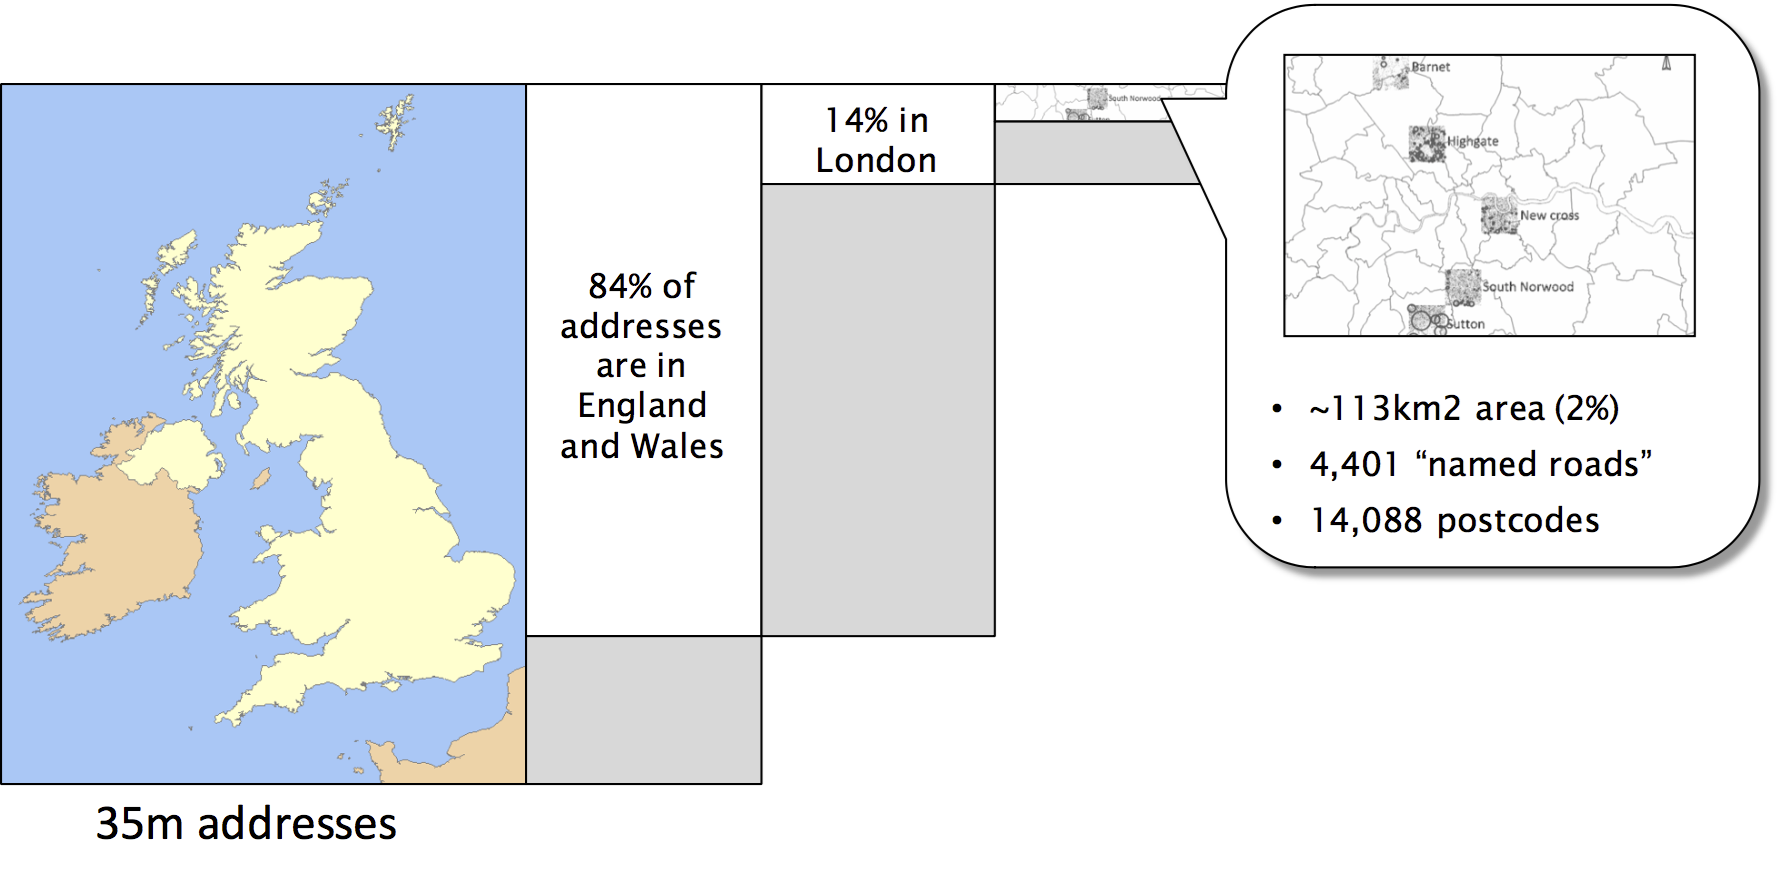
\includegraphics[width=0.50\textwidth]{social-machine-mix-3.png}}{\caption{Applicability of address inference - General statistics}\label{fig:social_machine_mix_3}}
        \ffigbox{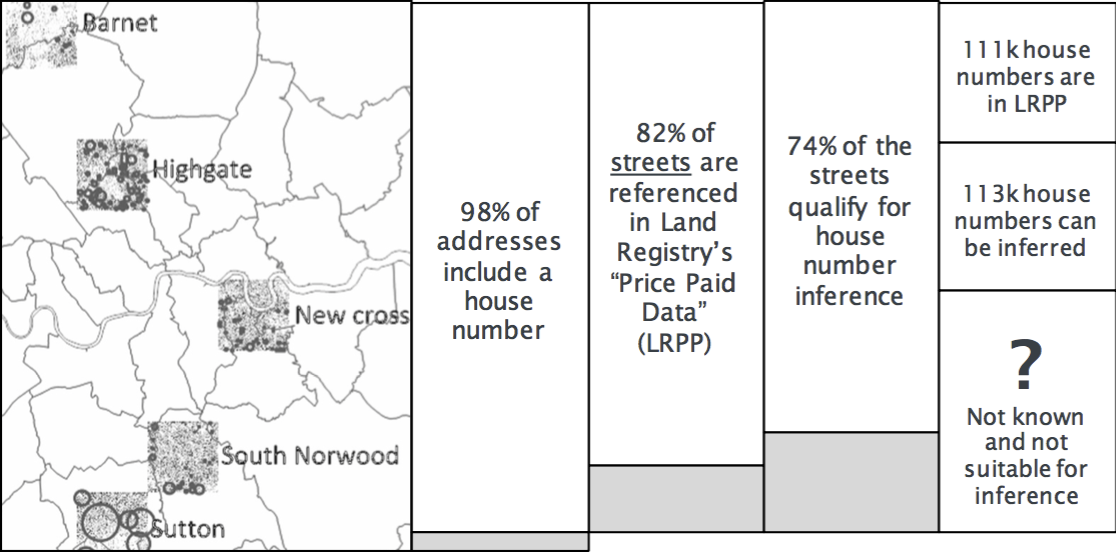
\includegraphics[width=0.40\textwidth]{social-machine-mix-2.png}}{\caption{Applicability of address inference - Sample statistics}\label{fig:social_machine_mix_2}}
   \end{floatrow}
\end{figure}
        
\textbf{Enabling inference for roads for which no house numbers are known} The focus going forward is on the latter problem. Using inference to create the largest sets of inferred house numbers translates into finding out the lowest and highest house numbers the algorithms could be applied to\footnote{For simplicity, we did not consider (a) that it is also useful to know if the streets have both odd and even house numbers and (b) the case where one house number only is known for a street, for which we could assume 1 to be the lowest house number.}.

As no pre-existing open data is available by definition to address this problem, the needed data needs being generated through surveying. 

\subsection{Crowdsourcing house numbers}

The crowdsourcing component of the platform can be configured to create the house numbers needed to enable inference. 

\begin{figure}
	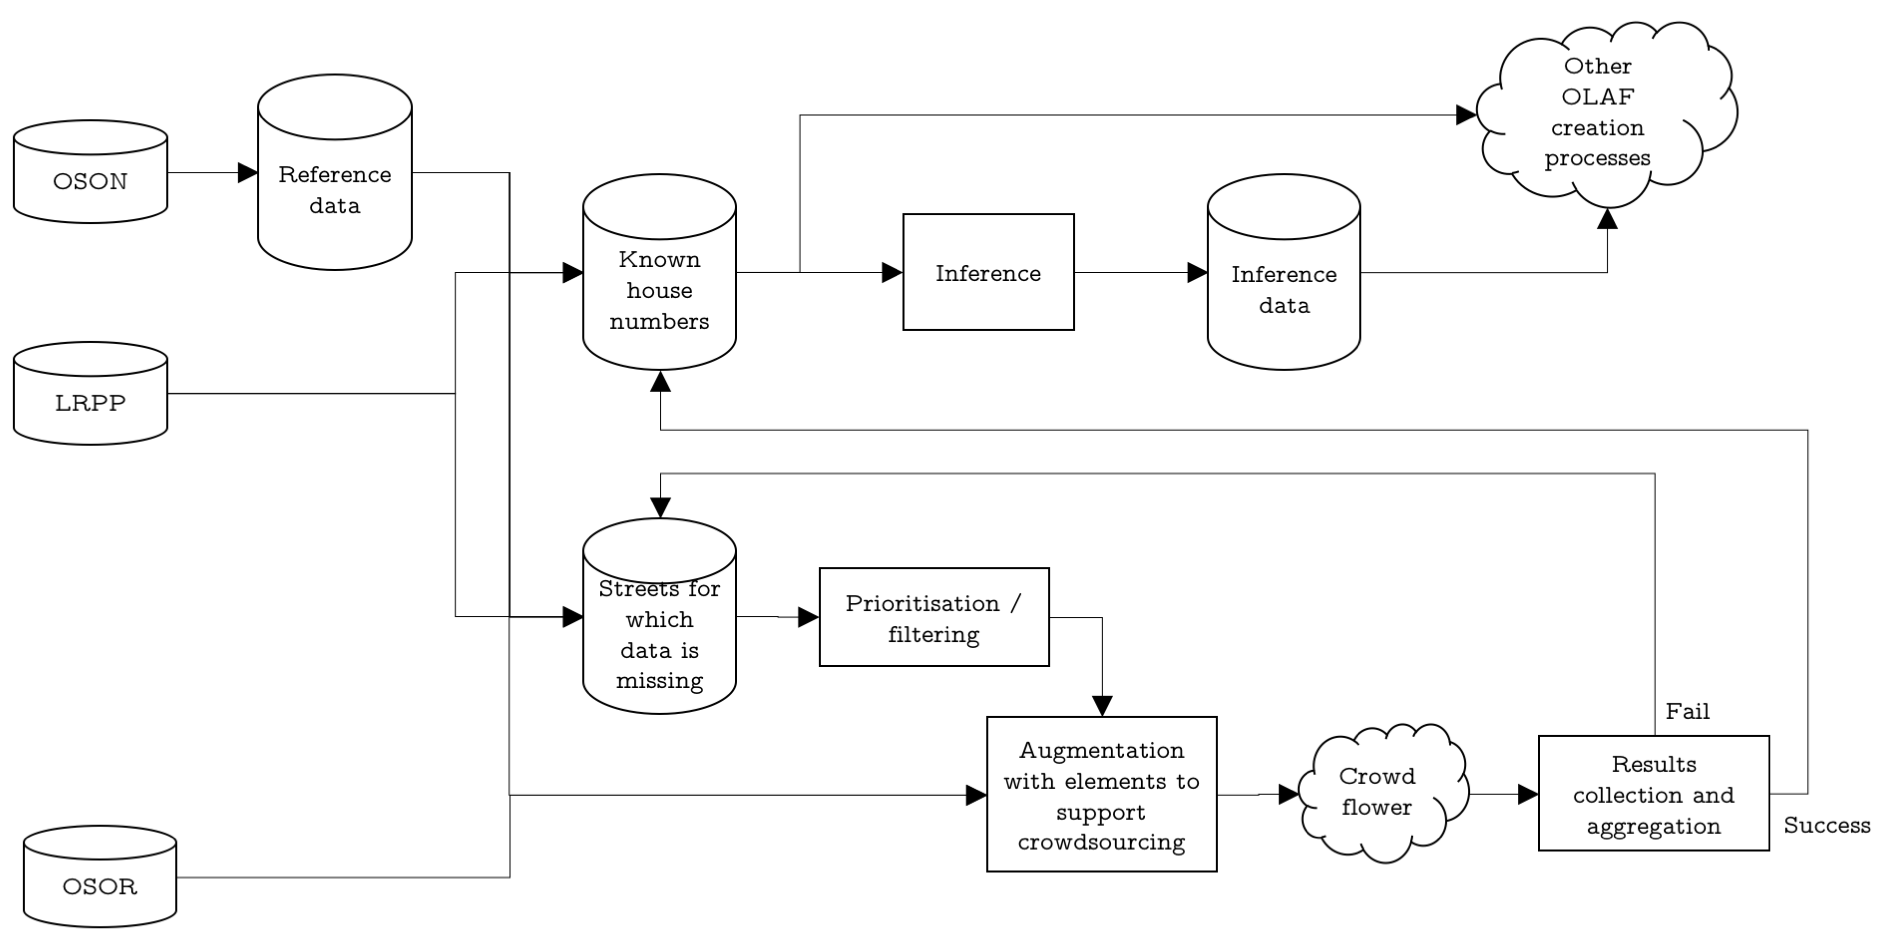
\includegraphics[width=1.0\textwidth]{workflow-1.png}
	\caption{Crowdsourcing house numbers in context}
	\label{fig:workflow_1}
\end{figure}

Observing the imagery of a street to identify its lowest and highest house number is not conceptually different than crowdsourced annotation applications that extensively studied in literature. 

It is worth though to highlight a few differences, though:

\begin{itemize}
        
    \item For each item subject to annotation, two independent\footnote{One could argue that the two annotations are not truly independent, as the lowest house number is, by definition, lower than the highest house number. In practical terms, though, the task of surveying a street cannot leverage such mathematical relation. In other words, knowing what the highest house number is won't help the participant finding the lowest house number, as her finding is rather due to the observation of the topology of the street and the progression of nearby house numbers.} annotations rather than one are collected: the lowest and highest visible house numbers\footnote{It is not useful to as a participant to look for the lowest house number and another to look for the highest. By exploring the pictures, participants will naturally focus her research on the extremities of the road, where the relevant house numbers are, without knowing in advance which of the two she is finding first.}.
        
    \item The information subject to the annotation could be identified as existing, but the annotation may not be possible anyway\footnote{E.g. a participant may be able to identify the first house in a street, but vegetation may hide the number. There is also the possibility that the mapping provider coverage does not include the surveyed street. Moreover, unlike other countries, in the UK local authorities do not provide house number plates to the building owners, so this remains their responsibility. Building owners have the option not to affix any plate at all.}.
        
    \item The road to survey may be no buildings\footnote{Because of how the workflow was defined, crowdsourcing is used on streets of which there is little or no reference in LRPP over the last 20 years. This means that the road is likely rural and have few buildings.}.
        
\end{itemize}
    
The following is a description of the approach that was used for crowdsourcing addresses, that is common to all experimental conditions that were tested.

\subsubsection{Task model} \leavevmode \\ %% Why is this necessary to get a new line?

\textbf{Requester.} The Requester desires to gather the lowest and the highest house numbers that can be observed in a specified street, as they can be intelligibly identified by browsing pictures of the street. Alternatively, if no two house numbers are identifiable, the Requester needs being informed, too. Different streets have different degree of interest to the Requester, who is interested in prioritising the collection of the data for the higher interest streets in respect to the lower interest ones. The Requester requires the help of human agents to carry out the tasks, that we will call Workers in the following.

\textbf{Task.} Each HIT (Human Intelligence Task) consists of browsing the pictures of a street until achieving reasonable certainty of having identified the lowest and the highest house numbers or, alternatively, the lack thereof.

\textbf{Strategy.} 
The strategy relies on traditional crowdsourcing techniques for image labelling.

\textbf{Crowd $\rightarrow$ Worker.} Each Worker provides judgement on a task by browsing the pictures and declaring if she has found the lowest and the highest house numbers or none. Multiple Workers are asked to identify the house numbers for the same street. The resulting data is chosen through majority voting. We use CrowdFlower as our crowdsourcing platform, presenting each task by embedding customised Google Maps and Google Street View applets into web pages built using the system's templating system. 

\textbf{Quality.} Quality is defined by a combination of (a) accuracy of the Workers in responding to tests questions, and (b) consensus in the data submitted through repeated surveys of the same road. Aggregation takes place accordingly as explained below.

\subsubsection{Workers quality}
    
Probing Workers using conventional test questions - e.g. where the correspondence of the Worker submissions is checked vs the same data collected by the research team as described in \cite{Kittur:2008gj} - would be a powerful tool to identify high vs low quality Workers, but is very expensive in OLAF's case. The task of surveying a street is not trivial, and early anecdotal evidence showed many Workers leaving after performing no more than two or three surveys. To further damage the performance of the system, the ones who stayed longer started cheating, or showed a substantial drop in their performance. This suggested that spending a substantial part of the Worker's effort on test questions - e.g. making one out of three surveys a test - was not affordable.

Not using any kind of test question is unlikely to be successful, too, and it was explored in previous work such as \cite{DellaPenna:tf} [THIS PAPER ACTUALLY THEORISES THE IMPOSSIBILITY OF GOOD RESULTS WHEN WORKERS HAVE ACCESS TO COMMONLY SHARED PREJUDICE: COULD THIS BE EQUIVALENT TO THE CASE WHERE MY WORKERS ALL END UP BELIEVING THAT SOME EASILY ACCESSIBLE AND VISIBLE CORNER OF A STREET HAS THE HIGHEST HOUSE NUMBER, BUT THE REAL ONE IS ELSEWHERE?]. As an alternative, though, simple test questions can be set up on data that is already available, in a way that is similar to classic anti-spamming techniques like CAPTCHAs as described in \cite{Difallah:2012ty}. In OLAF's case the name of the street itself is used: Workers are asked to copy and paste or type the name of the street as part of their survey. Workers that do not achieve the target accuracy are excluded from further work.

\subsubsection{Results aggregation}

Repeated surveys are equivalent to the use of repeated judgement in conventional image labelling exercises. These have been explored extensively in literature and demonstrate that the results produced by a few expensive expert individuals are comparable to what emerges from involving multiple answers by crowds of non-expert Workers, e.g. in \cite{Snow:2008wo} and \cite{Sheng:2008gra}. As the answers are inevitably noisy, different Workers were asked to survey the same road, and their responses are aggregated to decide what is the most likely and truthful observation. 
        
Approaches to aggregation are an equally well studied subject, and a majority decision is a natural option (e.g. \cite{Le:2010ug}). The detailed parameters and process of how consensus is defined and calculated are tuned for better performance and address issues specific to the context (e.g. in \cite{Hirth:2011fh}). 

In the case of OLAF, consensus is measured by using Fleiss' kappa statistics for inter-annotator agreement, as described for example in \cite{Nowak:2010gt}. For those streets where the house numbers {\it were} stated to be found, a kappa of 60\% on at least 5 surveys is sufficient consensus (e.g. see \cite{Landis:1977kv}). For those streets where the house numbers were stated {\it not} to be found, a kappa of 80\% on at least 10 surveys is required instead, as it is more likely that unreliable Workers agree in reporting that.

The number of 5 and 10 judgements is chosen because they are respectively the minimum number of judgements where 60\% and 80\% kappa can be achieved without the need of an unanimous agreement (4 vs 1 for 60\% and 9 vs 1 for 80\%). 

Rounds of 5 surveys per road are performed until consensus is reached on both its lowest and highest house numbers. Because of the nature of the task, new surveys are performed even if consensus is reached already on either of the two numbers.  

\subsubsection{Recruitment}

We sourced all our Workers from CrowdFlower. For each experiment, we created one dedicated CrowdFlower job. We used identical settings for each experiment set, consisting of the following parameters:

\textbf{Geography} Limited to the top 10 contributor countries in CrowdFlower where English is an official or officially recognised language\footnote{See \url{https://success.crowdflower.com/hc/en-us/articles/202703345-Crowd-Demographics}, the identification of the countries was last repeated on 19 December 2015, before the running the experiments described in this paper. The list of countries is: Bangladesh, Canada, India, Malaysia, Netherlands, Pakistan, Philippines, Sri Lanka, United Kingdom and United States of America.}.

\textbf{Skills} We chose Workers from the default CrowdFlower performance category (formerly named "level 2"), that accounts for 29\% of the total population\footnote{See \url{https://success.crowdflower.com/hc/en-us/articles/202703345-Crowd-Demographics}, the calculation was done on 19 December 2015.}[MORE INTERESTING TO KNOW THE VOLUME OF JUDGEMENTS THEY MAKE, THE OLDER CROWDFLOWER UI SEYI USED GAVE THIS INFORMATION].

\textbf{Accuracy} As described in the previous section, as a test question Workers were asked to copy and paste or type the name of the street as part of their submission in each task. Being the question this simple, error was not accepted the requested accuracy was 99\%\footnote{CrowdFlower does not allow the Requester to set target accuracy to 100\%.}.

\textbf{Judgements} In groups of 3 per road, repeated until consensus is reached, by different Workers without repetition. Each worker is allowed to contribute to a maximum of 10\% of the streets available to survey at each round.

\textbf{Behaviour} Each Worker was paid for 1 task, and 1 task is made of 1 street to survey.

\textbf{Reward / Time Limits} The reward was 0.20 US Dollars per task. Workers requiring less than 90 seconds per task were considered at high risk of being malicious and excluded to perform additional tasks. CrowdFlower imposes a time limit of 30 minutes maximum per task.

[TEXT REVISED UP TO HERE]

\subsection{Implementation}

(i) ingestion and preparation of the reference data\footnote{See the GitHub repository at \url{https://github.com/Digital-Contraptions-Imaginarium/OLAF-yr2_reference_data}.}, (ii) inference of house numbers where made possible from LRPP data\footnote{See the GitHub repository at \url{https://github.com/Digital-Contraptions-Imaginarium/OLAF-yr2_inference_data}.} and (iii) creation of the data for the crowdsourcing component and elaborating its results\footnote{See the GitHub repository at \url{https://github.com/Digital-Contraptions-Imaginarium/OLAF-yr2_lab}, {\it data-prep-scripts} and {\it analysis-scripts} folders respectively.}. 

[FIND SOME PLACE TO SAY WHY WE DON'T USE OPENSTREETMAP, BECAUSE SOMEONE WILL ASK. THE ANSWER IS THAT ITS LICENSING IS CONTROVERSIAL ACCORDING TO SOME: E.G. READ \cite{CentreforSpatialLawandPolicy:2014tx}]
    

